\subsection{Short Discussion about Rotational Transform $\iota$}
Imagine a magnetic confinement machine with only toroidal magnetic field. Since the magnetic field changes direction, there is a gradient (or some call it curvature, but they both serve the same purpose). From single particle in electromagnetic field demonstrations, you should know that if there is a gradient, there should be a $\nabla \B \times \B$ drift. For the tokamak shape, the gradient $\nabla \B$ is in $\hat{r}$ so radial direction, and the magnetic field itself, as assumed, is in $\hat{\phi}$ direction. From the cross product, this will result in upward or downward motion for ions and electrons. So, the charges will be separated. This separation will induce an electric field in the vertical direction $-\hat{z}$. And again from single particle motion, there will be a $\e\times \B$ drift. From cross product of $-\hat{z} \times \hat{\phi}$, the drift will be in radially outward $\hat{r}$ direction. Therefore, with only a toroidal magnetic field, we cannot confine charged particles.

A poloidal magnetic field is required for confinement, resulting in field lines which twist about flux surfaces. The twist in the field lines is quantified by the rotational transform, $\iota$, which indicates the number of poloidal turns of a field line around the magnetic axis for each toroidal turn around the $\hat{\textbf{z}}$ axis.
\begin{equation}
     \iota = \cfrac{B^{\theta^*}}{B^{\zeta}}
\end{equation}

Even if flux surfaces do not exist, the rotational transform can be defined with respect to the poloidal and toroidal rotation of a field line with respect to the magnetic axis. Often in the tokamak literature, the safety factor q = 1/$\iota$ is used rather than the rotational transform. If flux surfaces exist, the rotational transform can also be defined in terms of the fluxes as,
\begin{equation}
    \iota = \cfrac{\partial\psi_P/\partial\rho}{\partial\psi_T/\partial\rho}
\end{equation}

When the rotational transform is rational, $\iota$ = m/n for m and n integers, a field line closes on itself after n toroidal turns, having completed m poloidal turns. Therefore, a single field line does not cover the entire surface (see Figure \ref{rational-iota}). Flux surfaces with rational values of $\iota$ are known as rational surfaces. When $\iota$ is irrational, a given field line comes arbitrarily close to every point on what is called an irrational surface.
\begin{figure}[H]
    \centering
    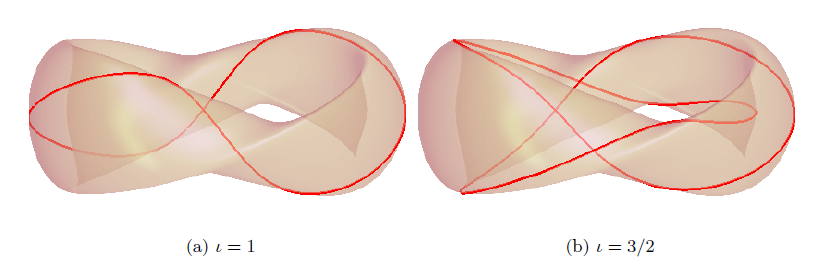
\includegraphics[height=4cm]{figures/rational-iota.png}
    \caption{Rational Transform Iota and Field lines closing on themselves \cite{imbert-gerard_introduction_nodate}}
    \label{rational-iota}
\end{figure}